\documentclass[../../course]{subfiles}

\renewcommand\thesection{\arabic{section}}


\begin{document}

\def\freqXOne{28}
\def\freqXTwo{56}
\def\freqXThree{56.1}

\def\sampFreqMuchLess{\textbf{(a):} $f_{s} = \frac{4 \times 28}{2} = 56 \si{Hz}$}
\def\sampFreqNorm{\textbf{(b):} $f_{s} = 4 \times 28 = 112 \si{Hz}$}
\def\sampFreqSligGreat{\textbf{(c):} $f_{s} = (4 \times 28) + 10 = 122 \si{Hz}$}
\def\sampFreqMuchGreat{\textbf{(d):} $f_{s} = 4 \times 28 \times 6 = 672 \si{Hz}$}

\section{Taking DFT of the Complex Sequences} \label{sec:wrkTakingDFTCplxSeqs}

In the previous Section, we took \textsc{DTFT}s of the \emph{sequences} we have
generated. In this Section, we will be taking \textsc{DFT}s of those same signals
and we can compare our findings. But before that let's take a look at what \textsc{DFT}s
are, and how to compute them.

\subsection{Discrete Fourier Transform}

Discrete Fourier Transforms or \textsc{DFT}s are just a special case of previously
mentioned \textsc{DTFT}s. \textsc{DTFT}s take a \emph{discrete} input sequence and
produces a \emph{continuous} signal. In the case of \textsc{DFT}, they take \emph{discrete}
input but produces a signal in the \emph{discrete} form itself. In other words, they
if we \emph{sample} \textsc{DTFT} we will get \textsc{DFT}. Mathematically they can
be described as,

\begin{align}
    X[k] &= X(e^{j\omega}) |_{\omega = \frac{2 \pi k}{N}} \\
    &= \sum_{n = 0}^{N - 1} x[n] e^{-j w n} \bigg|_{\omega = \frac{2 \pi k}{N}} \\
    &= \sum_{n = 0}^{N - 1} x[n] e^{\big(-j \frac{2 \pi k}{N} n \big)} \label{eqn:dftK}
\end{align}

where,

\begin{itemize} [label=]
    \item $X[k]$: is the \textsc{DFT} itself.

        where,

        \begin{itemize} [label=]
            \item $k$: varies from $0$ to $N - 1$
        \end{itemize}

    \item $N$: is the total \emph{sample count}.
    \item $x[n]$: is the \emph{input sequence}.

\end{itemize}

\subsection{Implementing DFT using Python}

Just like we did with \textsc{DTFT}s let's implement a similar \mintinline{python}{dtf_factory}
that would take \emph{complex sequence} and returns a \emph{function} that can be called with
$k$ for each of the values of \textsc{DFT}.

%python/dft_factory.py%
\begin{minted}[breaklines, autogobble, mathescape] {python}
    import numpy as np

    def dft_factory(cplx_seq):

        sample_count = len(cplx_seq)
        def dft(k):
            sum = 0
            # see eq. ($\ref{eqn:dftK}$)
            for n, cplx in enumerate(cplx_seq):
                sum = sum + cplx * np.exp(-1j * 2 * np.pi * k * n / sample_count)
            return sum

        return dft
\end{minted}

Now we need the \mintinline{python}{cplx_factory} from the previous section.

%python/cplx_factory.py%
\begin{minted}[breaklines, autogobble, mathescape] {python}
    def cplx_factory(samp_freq, real_freq, imag_freq):
        samp_period = 1 / samp_freq
        return lambda n: np.sin(
            2 * np.pi * real_freq * (n * samp_period)
        ) + 1j * np.sin(
            2 * np.pi * imag_freq * (n * samp_period)
        )
\end{minted}

Now let's implement a \emph{function} similar to that of \mintinline{python}{gen_dtft_seq}
for \textsc{DFT} that will generate the \textsc{DFT} sequence for our \emph{complex sequences}.
Let us call it..., you guessed it, yes, the \mintinline{python}{gen_dft_seq}!

%python/gen_dft_seq.py%
\begin{minted}[breaklines, autogobble, mathescape] {python}
    def gen_dft_seq(
        samp_count, samp_freq, real_freq, imag_freq
        ):

        cplx_fn = cplx_factory(
            samp_freq = samp_freq,
            real_freq = real_freq,
            imag_freq = imag_freq
        )

        cplx_seq = np.ndarray(samp_count, dtype = np.cdouble)

        for i in range(samp_count):
            cplx_seq[i] = cplx_fn(i)

        freq = np.arange(samp_count)

        dft_fn = dft_factory(cplx_seq = cplx_seq)
        dft_seq = dft_fn(freq)

        # we need to scale freq back
        return freq * samp_freq / samp_count, dft_seq, cplx_seq
\end{minted}

Now that we have \mintinline{python}{gen_dft_seq}, next we need a to compute $32$
point \textsc{DFT}s using all of these functions.

%python/taking_dft_32.py%
\begin{minted}[breaklines, autogobble, mathescape] {python}
    import pandas as pd

    X = 28

    cplx_seqs = [
        {
            "name": "complex_a",
            "real_freq": X,
            "imag_freq": X,
            # we will fill this later, for taking 64 point DFT
            "sequences": {},
        },
        {
            "name": "complex_b",
            "real_freq": X,
            "imag_freq": 2 * X,
            "sequences": {},
        },
        {
            "name": "complex_c",
            "real_freq": X,
            "imag_freq": (2 * X) + 0.1,
            "sequences": {},
        },
        {
            "name": "complex_f",
            "real_freq": 2 * X,
            "imag_freq": (2 * X) + 0.1,
            "sequences": {},
        },
    ]

    samp_freqs = {
        "normal":           int(4 * X),
        "slightly_greater": int(4 * X + 6),
        "much_greater":     int(4 * X * 10),
        "much_lesser":      int(4 * X / 2),
    }

    samp_count = 32

    for cplx in cplx_seqs:

        for samp_freq in samp_freqs:

            freq, dft_seq, cplx_seq = gen_dft_seq(
                samp_count = samp_count,
                samp_freq = samp_freqs[samp_freq],
                real_freq = cplx["real_freq"],
                imag_freq = cplx["imag_freq"]
            )

            # keeping generated sequences for taking 64 point DFT
            cplx["sequences"][samp_freq] = cplx_seq

            data = pd.DataFrame(
                data = {
                    "real": dft_seq.real,
                    "imag": dft_seq.imag,
                },
                index = freq
            )

            data.to_csv(
                "../data/dft_" + cplx["name"] + "_" + samp_freq + "_32.csv",
                sep = " ", index_label = "freq"
            )
\end{minted}

Next thing to do is to convert the above $32$ sized samples to $64$ sized samples
by \emph{zero padding}. Then we need to find $64$ point \textsc{DFT}s. Let's quickly
implement another \emph{function} called \mintinline{python}{gen_dft_seq_64}

%python/gen_dft_seq_64.py%
\begin{minted}[breaklines, autogobble, mathescape] {python}
    def gen_dft_seq_64(
        cplx_seq, samp_freq
        ):

        cplx_seq = np.concatenate(
            [cplx_seq, np.zeros(32, dtype = np.cdouble)]
        )

        freq = np.arange(64)

        dft_fn = dft_factory(cplx_seq = cplx_seq)
        dft_seq = dft_fn(freq)

        # we need to scale freq back
        return freq * samp_freq / 64, dft_seq, cplx_seq
\end{minted}

Now let's take the \textsc{DFT}s of our sequences using \mintinline{python}{gen_dft_seq_64}.

%python/taking_dft_64.py%
\begin{minted}[breaklines, autogobble, mathescape] {python}
    for cplx in cplx_seqs:
        for seq_name in cplx["sequences"]:
            freq, dft_seq, _ = gen_dft_seq_64(
                cplx_seq = cplx["sequences"][seq_name],
                samp_freq = samp_freqs[seq_name]
            )

            data = pd.DataFrame(
                data = {
                    "real": dft_seq.real,
                    "imag": dft_seq.imag,
                },
                index = freq
            )

            data.to_csv(
                "../data/dft_" + cplx["name"] + "_" + seq_name + "_64.csv",
                sep = " ", index_label = "freq"
            )
\end{minted}

\pagebreak

\subsection{DFT of Complex A} \label{ssec:dtftCplxA}

\begin{itemize} [label=]

    \item \textbf{Sequence:} $\sin(2 \pi \freqXOne t) + j \sin(2 \pi \freqXOne t)$

\end{itemize}

\subsubsection{DFT with 32 Samples}

\begin{itemize} [label=]

    \item \sampFreqMuchLess
        \begin{itemize} [label=]
            \item There is no \emph{hope} in \emph{alias land}, we could see
                something between $25$ $30$.
        \end{itemize}

    \item \sampFreqNorm
        \begin{itemize} [label=]
            \item We could see a spike at somewhat near the vicinity of $\freqXOne \si{Hz}$.
        \end{itemize}

    \item \sampFreqSligGreat
        \begin{itemize} [label=]
            \item There is a little bit of bulge can be seen near $\freqXOne \si{Hz}$.
        \end{itemize}

    \item \sampFreqMuchGreat
        \begin{itemize} [label=]
            \item There is little bit bulge at the left end.
        \end{itemize}

    \item \textbf{Inference:} It seems like if we only increase the \emph{sampling frequency},
        but keep the \emph{sample count} same, the \emph{uncertainty} also increases.

\end{itemize}

\vfill

\begin{figure} [H]
    \centering
    \adjustbox{max width = 1\textwidth} {
        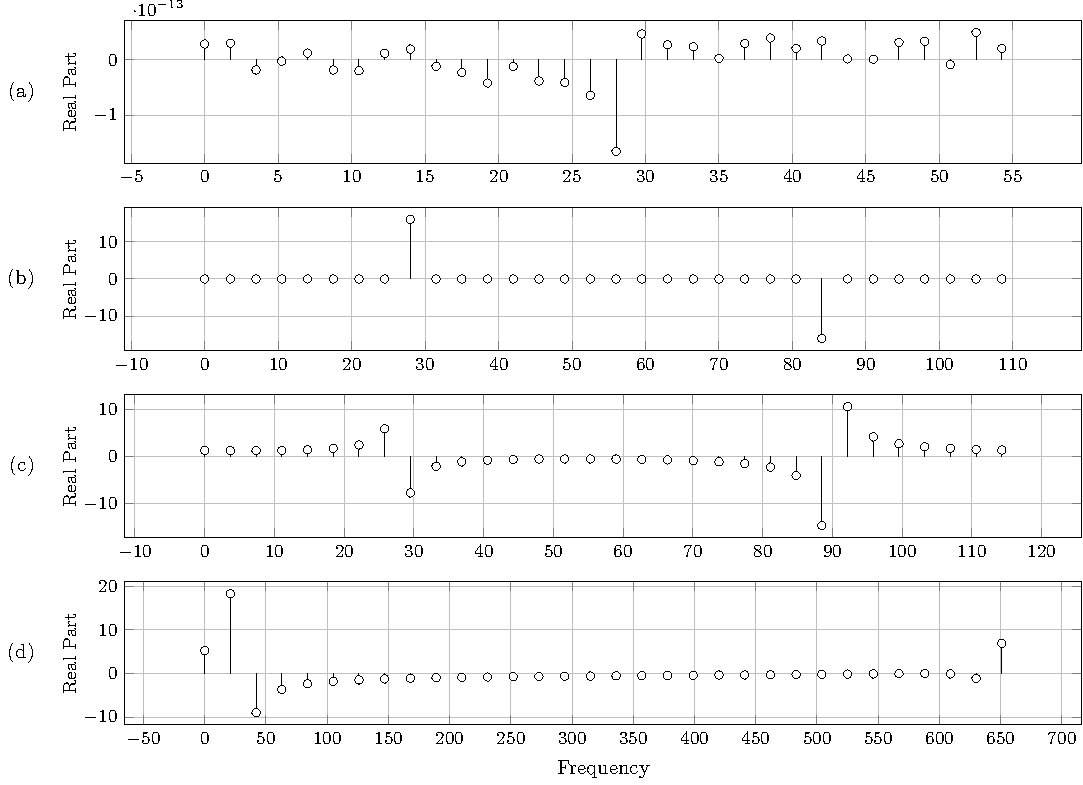
\includegraphics[height = 0.8\textheight] {tikzpics/plotDftComplexA32.pdf}
    }
    \captionof{figure} {Plot of \textsc{DFT}s of \textsc{Complex A} with different sampling frequencies}
    \label{plt:dftComplexA}
\end{figure}

\subsubsection{DFT with 64 Samples}

\begin{itemize} [label=]

    \item \sampFreqMuchLess
        \begin{itemize} [label=]
            \item
        \end{itemize}

    \item \sampFreqNorm
        \begin{itemize} [label=]
            \item
        \end{itemize}

    \item \sampFreqSligGreat
        \begin{itemize} [label=]
            \item
        \end{itemize}

    \item \sampFreqMuchGreat
        \begin{itemize} [label=]
            \item
        \end{itemize}

    \item \textbf{Inference:} Surprisingly, $64$ point increases the resolution to \emph{double}. And we
        can now see more information from the \emph{spectrum}.

\end{itemize}

\vfill

\begin{figure} [H]
    \centering
    \adjustbox{max width = 1\textwidth} {
        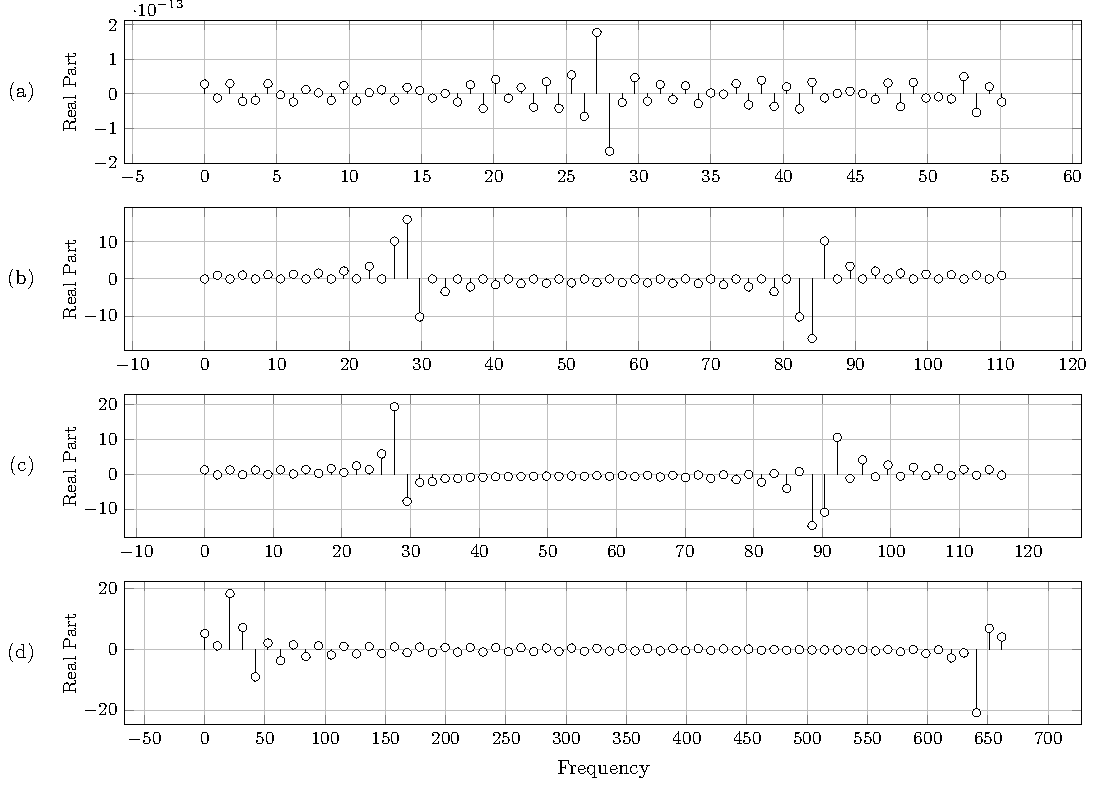
\includegraphics[height = 0.8\textheight] {tikzpics/plotDftComplexA64.pdf}
    }
    \captionof{figure} {Plot of \textsc{DFT}s of \textsc{Complex A} with different sampling frequencies}
    \label{plt:dftComplexA}
\end{figure}

\pagebreak

\subsection{DFT of Complex B} \label{ssec:dtftCplxB}

\begin{itemize} [label=]

    \item \textbf{Sequence:} $\sin(2 \pi \freqXOne t) + j \sin(2 \pi \freqXTwo t)$

\end{itemize}

\subsubsection{DFT with 32 Samples}

\begin{itemize} [label=]

    \item \sampFreqMuchLess
        \begin{itemize} [label=]
            \item \emph{Alias land}, no hope.
        \end{itemize}

    \item \sampFreqNorm
        \begin{itemize} [label=]
            \item Could see some noise.
        \end{itemize}

    \item \sampFreqSligGreat
        \begin{itemize} [label=]
            \item We can kind of see two of the frequencies.
        \end{itemize}

    \item \sampFreqMuchGreat
        \begin{itemize} [label=]
            \item Uncertainty increases.
        \end{itemize}

    \item \textbf{Inference:} Same as \textsc{Complex A}.

\end{itemize}

\vfill

\begin{figure} [H]
    \centering
    \adjustbox{max width = 1\textwidth} {
        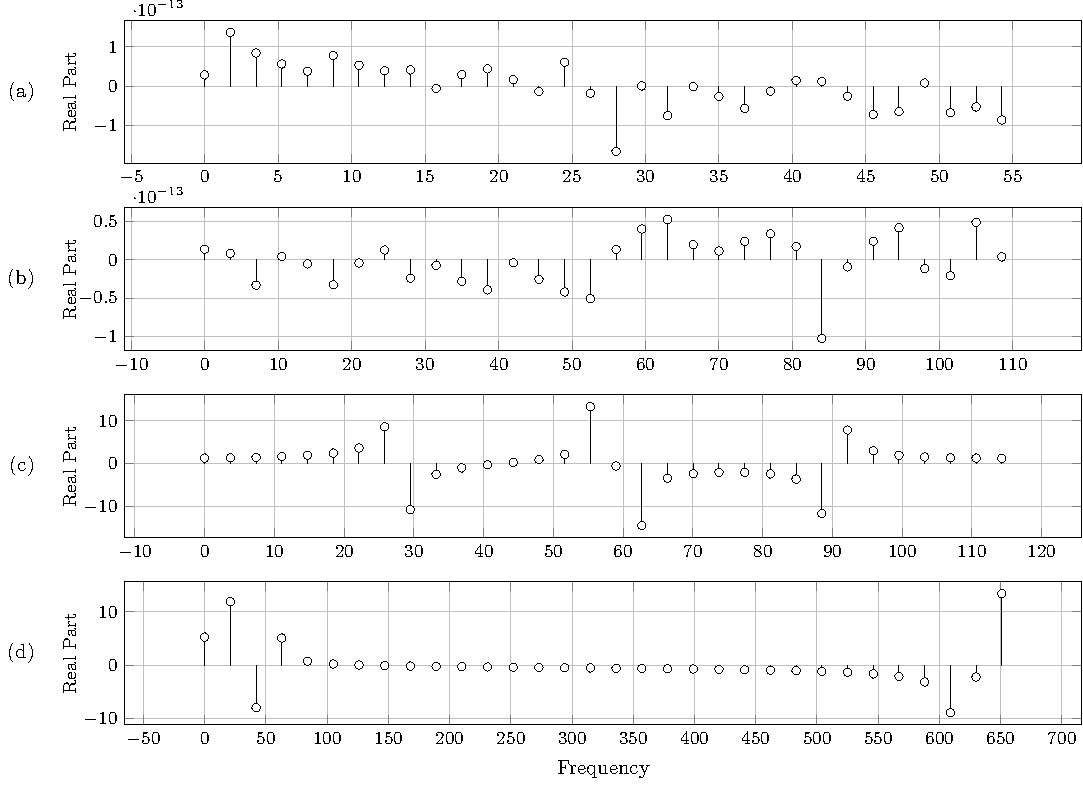
\includegraphics[height = 0.8\textheight] {tikzpics/plotDftComplexB32.pdf}
    }
    \captionof{figure} {Plot of \textsc{DFT}s of \textsc{Complex B} with different sampling frequencies}
    \label{plt:dftComplexB}
\end{figure}

\subsubsection{DFT with 64 Samples}

\begin{itemize} [label=]

    \item \sampFreqMuchLess
        \begin{itemize} [label=]
            \item
        \end{itemize}

    \item \sampFreqNorm
        \begin{itemize} [label=]
            \item
        \end{itemize}

    \item \sampFreqSligGreat
        \begin{itemize} [label=]
            \item
        \end{itemize}

    \item \sampFreqMuchGreat
        \begin{itemize} [label=]
            \item
        \end{itemize}

    \item \textbf{Inference:} Similar to \textsc{Complex A}. Doubles the resolution.

\end{itemize}

\vfill

\begin{figure} [H]
    \centering
    \adjustbox{max width = 1\textwidth} {
        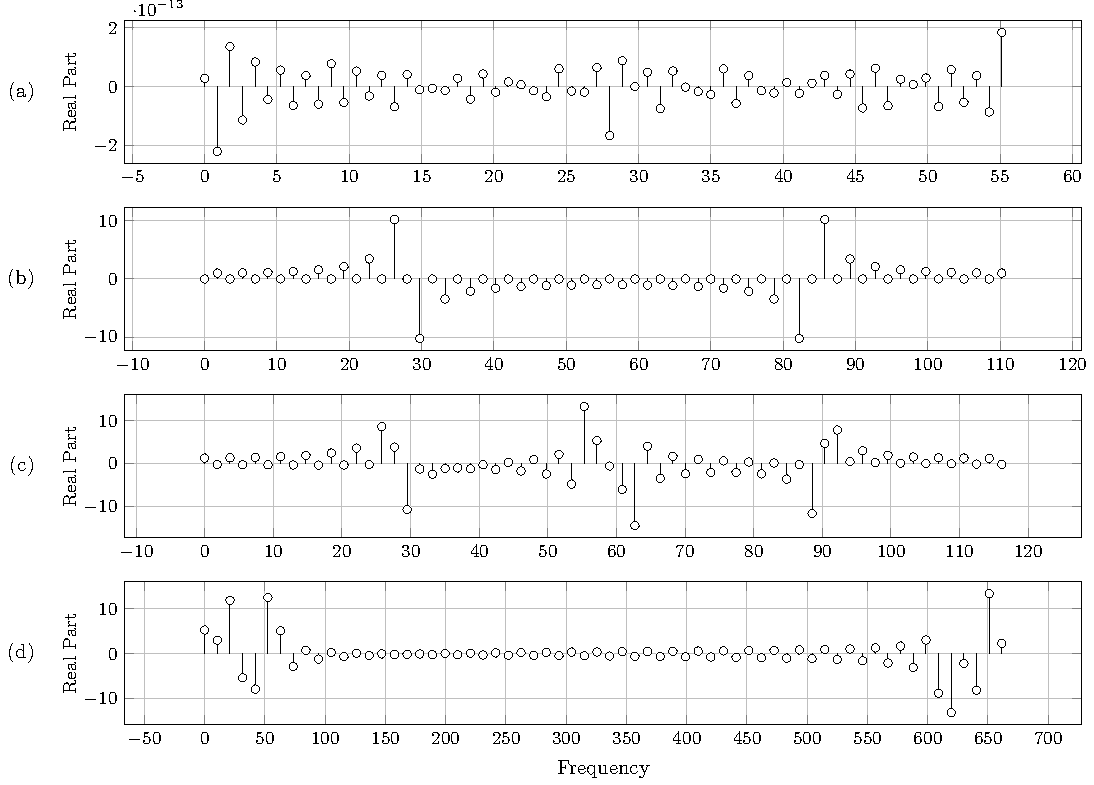
\includegraphics[height = 0.8\textheight] {tikzpics/plotDftComplexB64.pdf}
    }
    \captionof{figure} {Plot of \textsc{DFT}s of \textsc{Complex B} with different sampling frequencies}
    \label{plt:dftComplexB}
\end{figure}

\pagebreak

\subsection{DFT of Complex C} \label{ssec:dtftCplxC}

\begin{itemize} [label=]

    \item \textbf{Sequence:} $\sin(2 \pi \freqXOne t) + j \sin(2 \pi \freqXThree t)$

\end{itemize}

\subsubsection{DFT with 32 Samples}

\begin{itemize} [label=]

    \item \sampFreqMuchLess
        \begin{itemize} [label=]
            \item Aliasing causing, misinformation.
        \end{itemize}

    \item \sampFreqNorm
        \begin{itemize} [label=]
            \item Cant's see $\freqXOne \si{Hz}$ but something is present near the $50$s ranges.
        \end{itemize}

    \item \sampFreqSligGreat
        \begin{itemize} [label=]
            \item Can almost see both.
        \end{itemize}

    \item \sampFreqMuchGreat
        \begin{itemize} [label=]
            \item Similar as above.
        \end{itemize}

    \item \textbf{Inference:} Similar to above two \emph{sequences}.

\end{itemize}

\vfill

\begin{figure} [H]
    \centering
    \adjustbox{max width = 1\textwidth} {
        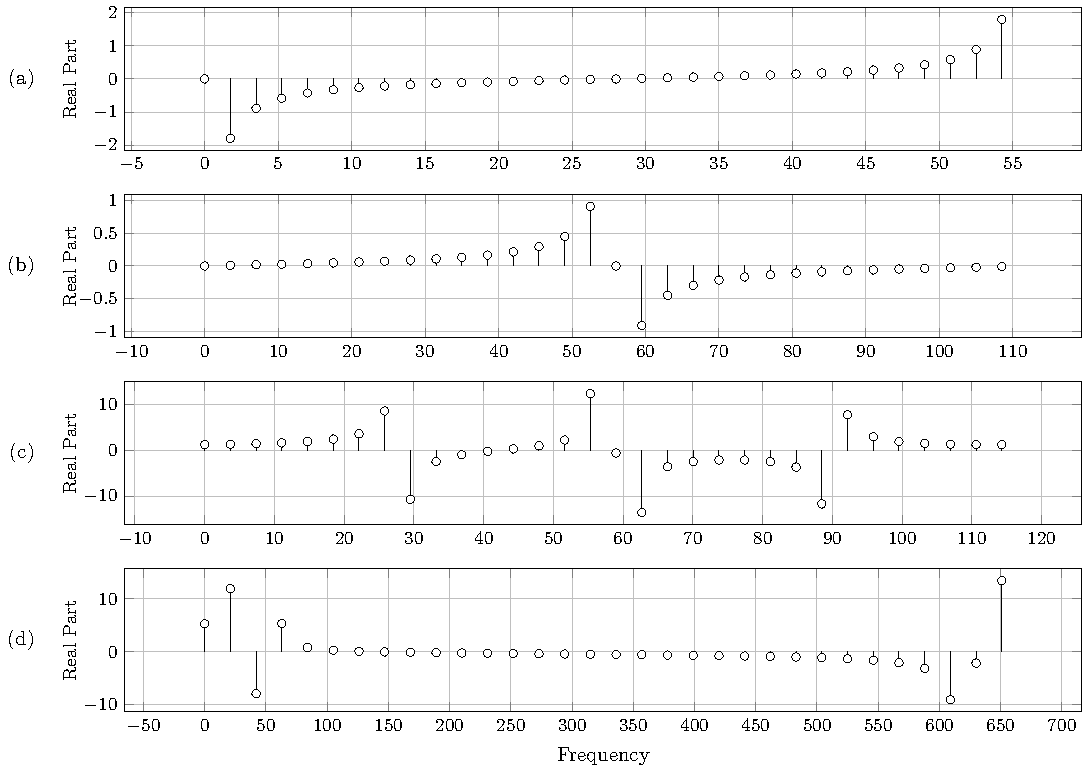
\includegraphics[height = 0.8\textheight] {tikzpics/plotDftComplexC32.pdf}
    }
    \captionof{figure} {Plot of \textsc{DFT}s of \textsc{Complex C} with different sampling frequencies}
    \label{plt:dftComplexC}
\end{figure}

\subsubsection{DFT with 64 Samples}

\begin{itemize} [label=]

    \item \sampFreqMuchLess
        \begin{itemize} [label=]
            \item
        \end{itemize}

    \item \sampFreqNorm
        \begin{itemize} [label=]
            \item
        \end{itemize}

    \item \sampFreqSligGreat
        \begin{itemize} [label=]
            \item
        \end{itemize}

    \item \sampFreqMuchGreat
        \begin{itemize} [label=]
            \item
        \end{itemize}

    \item \textbf{Inference:} Resolution increases, so does if there is \emph{aliasing}.

\end{itemize}

\vfill

\begin{figure} [H]
    \centering
    \adjustbox{max width = 1\textwidth} {
        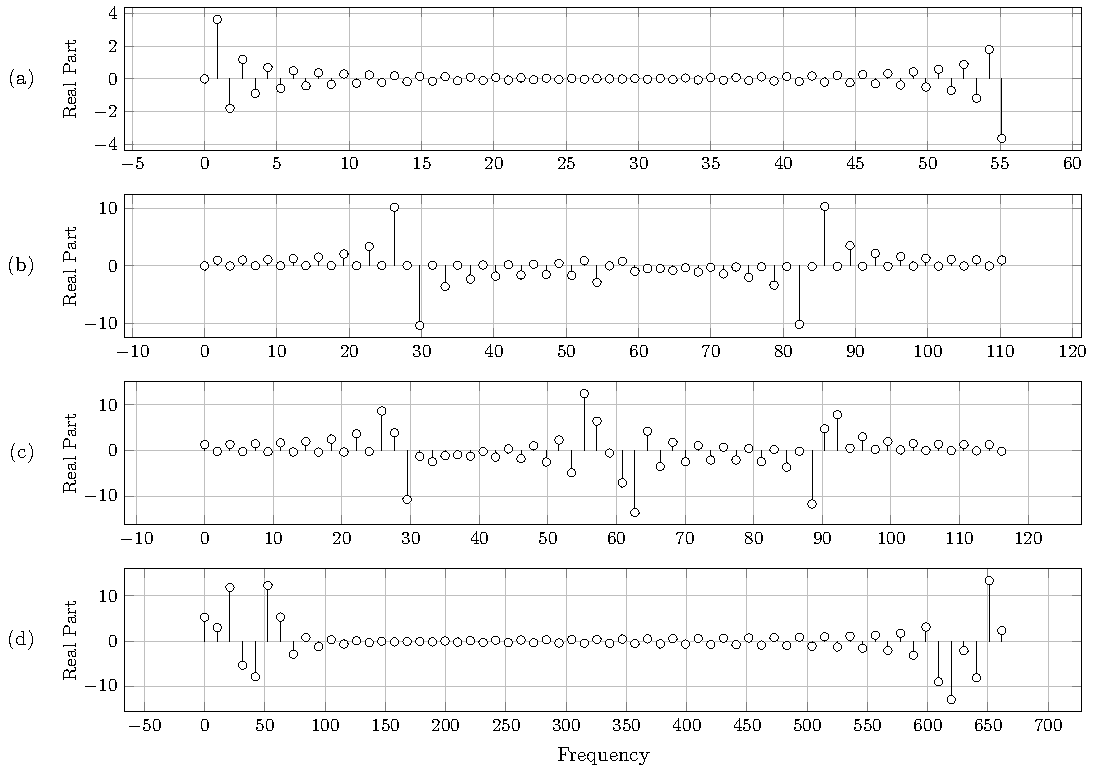
\includegraphics[height = 0.8\textheight] {tikzpics/plotDftComplexC64.pdf}
    }
    \captionof{figure} {Plot of \textsc{DFT}s of \textsc{Complex C} with different sampling frequencies}
    \label{plt:dftComplexC}
\end{figure}

\pagebreak

\subsection{DFT of Complex F} \label{ssec:dtftCplxF}

\begin{itemize} [label=]

    \item \textbf{Sequence:} $\sin(2 \pi \freqXTwo t) + j \sin(2 \pi \freqXThree t)$

\end{itemize}

\subsubsection{DFT with 32 Samples}

\begin{itemize} [label=]

    \item \sampFreqMuchLess
        \begin{itemize} [label=]
            \item \emph{Aliasing}.
        \end{itemize}

    \item \sampFreqNorm
        \begin{itemize} [label=]
            \item Unable to distinguish between two of the similar frequencies.
        \end{itemize}

    \item \sampFreqSligGreat
        \begin{itemize} [label=]
            \item Unable to distinguish between two of the similar frequencies.
        \end{itemize}

    \item \sampFreqMuchGreat
        \begin{itemize} [label=]
            \item Same as above.
        \end{itemize}

    \item \textbf{Inference:} Similar to above sequences.

\end{itemize}

\vfill

\begin{figure} [H]
    \centering
    \adjustbox{max width = 1\textwidth} {
        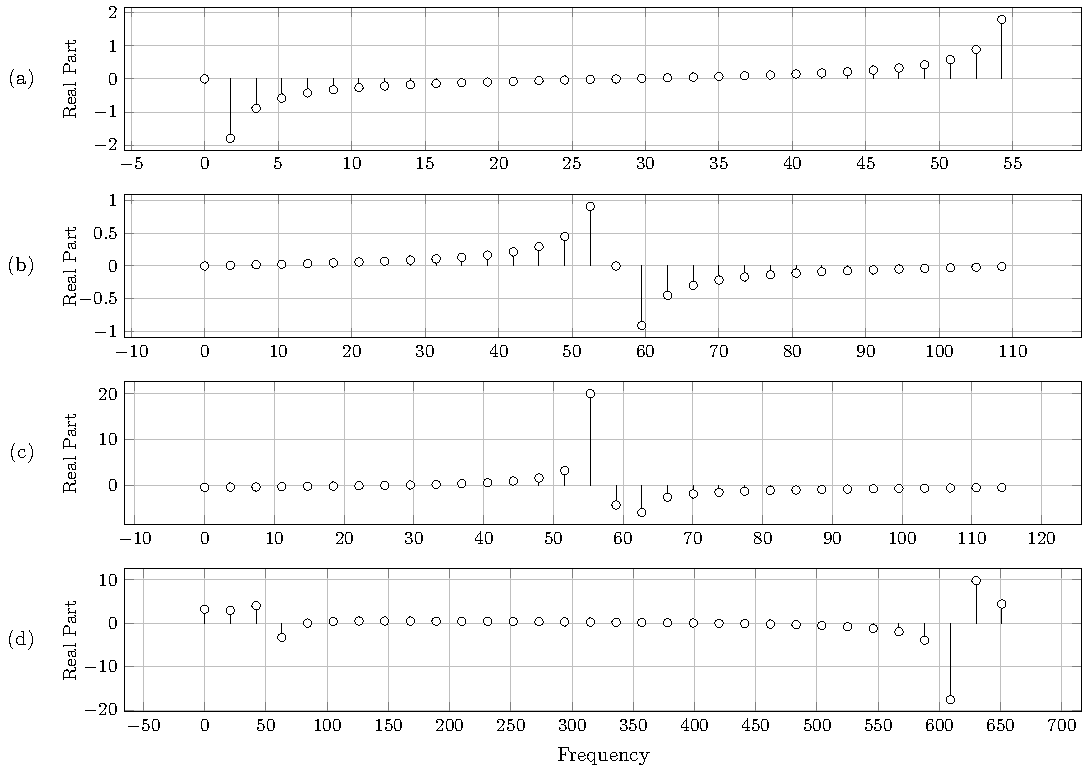
\includegraphics[height = 0.8\textheight] {tikzpics/plotDftComplexF32.pdf}
    }
    \captionof{figure} {Plot of \textsc{DFT}s of \textsc{Complex F} with different sampling frequencies}
    \label{plt:dftComplexF}
\end{figure}

\subsubsection{DFT with 64 Samples}

\begin{itemize} [label=]

    \item \sampFreqMuchLess
        \begin{itemize} [label=]
            \item
        \end{itemize}

    \item \sampFreqNorm
        \begin{itemize} [label=]
            \item
        \end{itemize}

    \item \sampFreqSligGreat
        \begin{itemize} [label=]
            \item
        \end{itemize}

    \item \sampFreqMuchGreat
        \begin{itemize} [label=]
            \item
        \end{itemize}

    \item \textbf{Inference:} Resolution increases.

\end{itemize}

\vfill

\begin{figure} [H]
    \centering
    \adjustbox{max width = 1\textwidth} {
        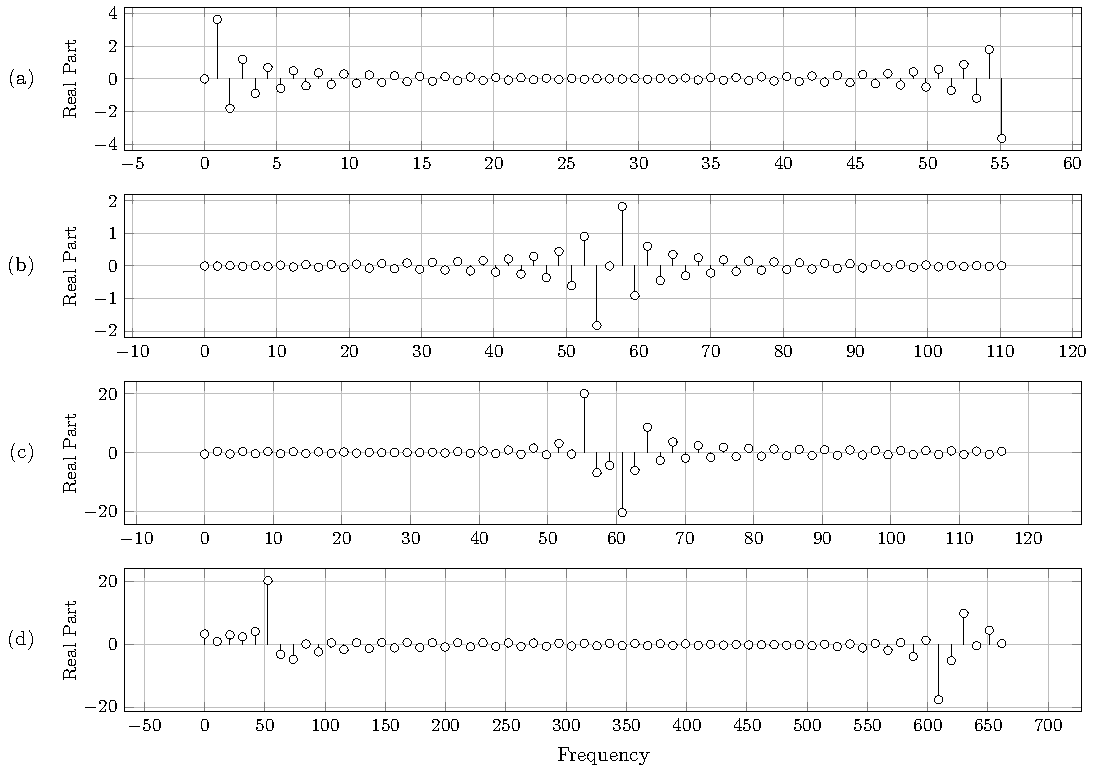
\includegraphics[height = 0.8\textheight] {tikzpics/plotDftComplexF64.pdf}
    }
    \captionof{figure} {Plot of \textsc{DFT}s of \textsc{Complex F} with different sampling frequencies}
    \label{plt:dftComplexF}
\end{figure}


\end{document}
